\begin{figure} [!ht]
\begin{center}
\begin{tikzpicture}
	[
	sibling distance=150pt,
	level distance=100pt,
	level 1/.style={sibling distance=6cm},
	level 2/.style={sibling distance=3cm},
	every node/.style = {
	},
	every child/.style = {
		ultra thick
	}
	]

\node[draw] (title) at (0, 1.5) {Game Tree};

\node {
	\begin{tikzpicture}
		\draw[] (0.6,-0.3) rectangle ++(0.3,0.3);
		\draw[] (0.9,-0.3) rectangle ++(0.3,0.3);
		\draw[] (0,-0.3) rectangle ++(0.3,0.3);
		\draw[] (0,0) rectangle ++(0.3,0.3);
		\draw[] (0.3,0) rectangle ++(0.3,0.3);
		\draw[] (0.6,0) rectangle ++(0.3,0.3);
		\draw[] (0.3,0.3) rectangle ++(0.3,0.3);
		\draw[] (0.6,0.3) rectangle ++(0.3,0.3);
		\draw[] (0,0.6) rectangle ++(0.3,0.3);
		\draw[] (0.3,0.6) rectangle ++(0.3,0.3);
		\draw[] (0.6,0.6) rectangle ++(0.3,0.3);
	\end{tikzpicture}}
child {node { 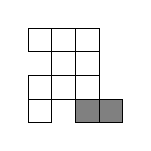
\begin{tikzpicture}
	\draw[fill=gray] (0.6,-0.3) rectangle ++(0.3,0.3);
	\draw[fill=gray] (0.9,-0.3) rectangle ++(0.3,0.3);
	\draw[] (0,-0.3) rectangle ++(0.3,0.3);
	\draw[] (0,0) rectangle ++(0.3,0.3);
	\draw[] (0.3,0) rectangle ++(0.3,0.3);
	\draw[] (0.6,0) rectangle ++(0.3,0.3);
	\draw[] (0.3,0.3) rectangle ++(0.3,0.3);
	\draw[] (0.6,0.3) rectangle ++(0.3,0.3);
	\draw[] (0,0.6) rectangle ++(0.3,0.3);
	\draw[] (0.3,0.6) rectangle ++(0.3,0.3);
	\draw[] (0.6,0.6) rectangle ++(0.3,0.3);
\end{tikzpicture}}}
child {node {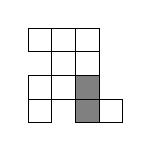
\begin{tikzpicture}
	\draw[fill=gray] (0.6,-0.3) rectangle ++(0.3,0.3);
	\draw[] (0.9,-0.3) rectangle ++(0.3,0.3);
	\draw[] (0,-0.3) rectangle ++(0.3,0.3);
	\draw[] (0,0) rectangle ++(0.3,0.3);
	\draw[] (0.3,0) rectangle ++(0.3,0.3);
	\draw[fill=gray] (0.6,0) rectangle ++(0.3,0.3);
	\draw[] (0.3,0.3) rectangle ++(0.3,0.3);
	\draw[] (0.6,0.3) rectangle ++(0.3,0.3);
	\draw[] (0,0.6) rectangle ++(0.3,0.3);
	\draw[] (0.3,0.6) rectangle ++(0.3,0.3);
	\draw[] (0.6,0.6) rectangle ++(0.3,0.3);
\end{tikzpicture}}};

\end{tikzpicture}
\end{center}
\end{figure}